%
% ebene.tex
%
% (c) 2018 Prof Dr Andreas Müller, Hochschule Rapperswil
%
\documentclass[tikz,12pt]{standalone}
\usepackage{times}
\usepackage{amsmath}
\usepackage{txfonts}
\usepackage[utf8]{inputenc}
\usepackage{graphics}
\usetikzlibrary{arrows,intersections,math}
\usepackage{ifthen}
\begin{document}

\newboolean{showgrid}
\setboolean{showgrid}{false}

\begin{tikzpicture}[>=latex,thick]

% Povray Bild
\node at (0,0) {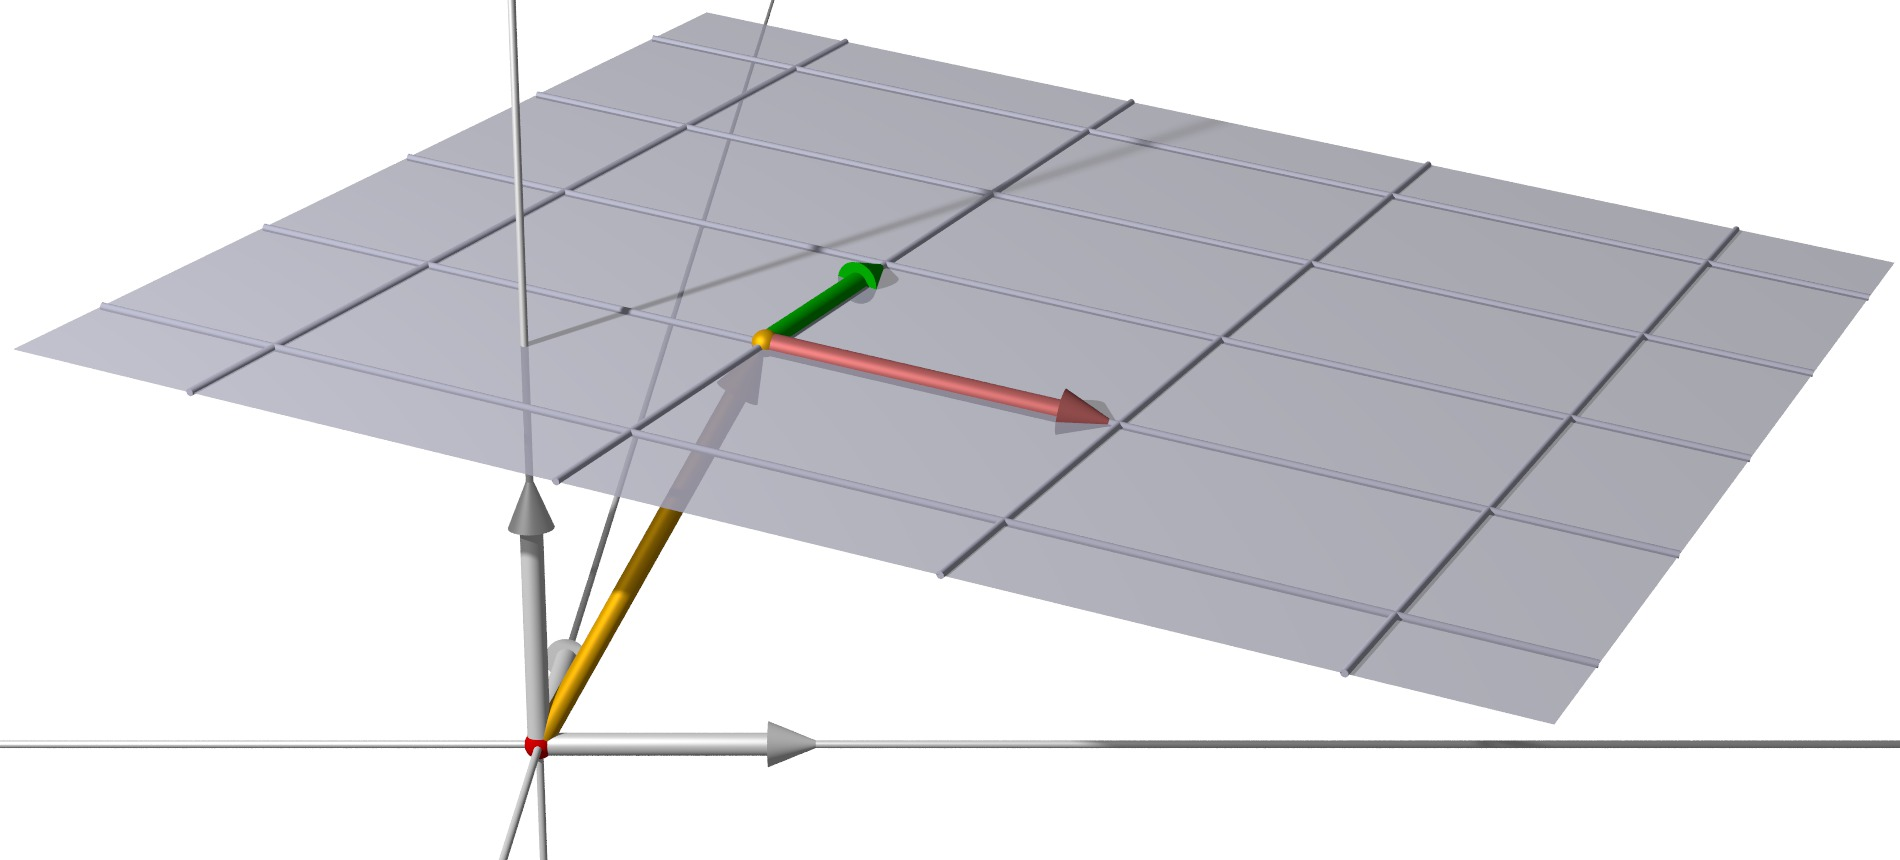
\includegraphics[width=14cm]{ebene.jpg}};

% Gitter
\ifthenelse{\boolean{showgrid}}{
\draw[step=0.1,line width=0.1pt] (-7,-3) grid (7, 3);
\draw[step=0.5,line width=0.4pt] (-7,-3) grid (7, 3);
\draw (-7,-3) grid (7, 3);
\fill (0,0) circle[radius=0.05];
}{}

% Ursprung
\node at (-3.36,-2.6) {$O$};

% Richtungs-Vektoren
\node at (1.26,0.42) {$\vec{u}$};
\node at (-0.56,1.54) {$\vec{v}$};

% Stützvektor
\node at (-1.54,0.98) {$P$};
\node at (-1.96,-0.98) {$\vec{p}$};

% Ebene
\node at (4.5,1.05) {$\sigma$};

\end{tikzpicture}

\end{document}

